\chapter{Method} \label{cha:Method}

\section{Introduction} \label{sec:Method-intro}

This chapter first explains the different software packages used throughout this project, and then outlines the recommended procedure to determine a suitable trajectory for \BW\ once the launch details and configuration are confirmed.

% Procedure
\section{Developmental procedure} \label{sec:Development}

\subsection{Matlab modelling} \label{sub:Matlab}

As mentioned in \autoref{sec:Numerical-considerations}, early in the project the orbital mechanics of \autoref{cha:Orbital-dynamics-and-modelling} were modelled in Matlab to verify the flight mechanics and resolve numerical issues associated with long-duration integration and frame conversion. Matlab's native optimisation procedures were examined, but found inadequate for the number of variables required.

\subsection{GESOP modelling} \label{sub:GESOP}

Development was then transferred to GESOP. The model library and graphical front-end ASTOS was briefly used but found to be far to restricting for a problem of this complexity. Consequently the vehicle and orbital mechanics were coded to the C interface available within GESOP. In addition to encapsulating several optimisation procedures, GESOP provided automatic mesh generation as explained in \autoref{sub:Discretisation}, given appropriate error tolerances as explained in \autoref{sub:Integration-error}.

To get an initial idea of the optimal thrust profile, first a reduced complexity ascent trajectory was modelled. This was implemented simply by deactivating secondary and tertiary perturbations, and optimising over a coarse mesh. As a result, this phase was quickly able to reach an optimal solution, giving an idea of the optimal results that would have resulted in the other phases given adequate computing power. Many useful observations were drawn from this preliminary optimised trajectory, so the results have been included in \autoref{cha:Results}.

Following the reduced complexity ascent, optimisation was attempted for a reduced complexity cruise phase. However, due to the long duration of this phase and the limited computer resources available, the optimisation did not reach an optimal solution in the time available. This exercise did highlight other problems with the procedure, in particular determining a lunar capture. Due to the lunar orbit being very close to the orbital escape energy relative to the Earth (only $5\times10^5$~m$^2$s$^{-2}$), the vast majority of simulations resulted in the spacecraft escaping the Earth's sphere of influence by gaining a gravitational assist from the Moon. This caused severe computational errors as the longitude and anomaly are no longer independent parameters after escape. Another common failure scenario involved weak capture by the Moon; after one or two orbits around the Moon the spacecraft would then be recaptured by the Earth. Due to the way the system was modelled, this once again caused computational errors: if the spacecraft is in orbit around the Moon in a Earth-centric frame, the anomaly becomes sinusoidal rather than always increasing; the same applies for a spacecraft in Earth orbit during a lunar-centric frame.

Determining conditions for strong lunar capture proved difficult and unreliable. Consequently it was decided to simulate the transfer backwards, from lunar orbit to Earth orbit, using an industry standard tool called Satellite Tool Kit (STK)%\parencite{STK}
. Backwards propagation has been used by many previous authors, such as \textcite{Kluever1995}. The main advantage to this approach is that any ascent from lunar orbit must necessarily pass through Earth orbit, whereas the reverse does not apply. Furthermore, with the Moon in a 19\degrees\ inclined orbit about the Earth, any ascent from the Moon will end up in approximately the same plane as the parking orbit after launch, thus implicitly accounting for the plane changes required to achieve the target lunar orbit. Backwards propagation is particularly well suited to this real-world application, because once the payload mass is finalised backwards propagation allows exact determination of the wet mass required.

\subsection{STK modelling} \label{sec:STK}

As outlined above, the Satellite Tool Kit (STK), provided by AGI (Analytical Graphics, Inc.), was chosen to model the trajectory. STK is widely used in industry for defence and space simulation, and has developed an extensive collection of features. Recent developments have even included an optimiser for interplanetary trajectories. Unfortunately, the native optimiser still only supports a very limited number of optimisable parameters, for example the direction and magnitude of an impulsive burn to perform a trans-lunar injection. The high number of parameters resulting from discretisation of a continuous trajectory is, for the moment, beyond the capabilities of STK, even to the extent of solving the 2-point boundary value problem (in other words, STK cannot find a feasible solution to the problem let alone optimise it).

Therefore STK cannot target a specific orbit, such as the correct inclination and eccentricity of the GTO (after backwards propagating from LLO). However, as stated above, the fact that any ascent from the Moon passes through Earth orbit, with an inclination of approximately 19\degrees\ means that it can be a very useful tool to study lunar capture. A number of backwards propagations were performed, mostly resulting in escape orbits. However, by manipulating the start date and anomaly, it was found that some \enquote{ascents} would put the spacecraft into a stable Earth orbit (provided the thrust stops once lunar escape is achieved). From this point a geocentric frame of reference could be implemented and the PPTs could lower the orbital radius of the spacecraft relative to the Earth. Once the PPT \enquote{descent} reaches the van Allen belts for the first time, this is equivalent to the last time the spacecraft would be within the van Allen belts in the chronologically correct simulation, and consequently defines the phase boundary perfectly.

Due to the limited number of optimisable parameters, the thrust vector must be easily defined relative to one of the STK frames. For the purposes of this simulation, the thrust vector was defined to be negative velocity for the lunar phases, and positive velocity for the geocentric phases. One of the resulting trajectories is shown in \autoref{fig:STK}. The trajectory smoothly \enquote{ascends} from LLO by thrusting along the negative velocity vector, transitions cleanly into Earth orbit, and then \enquote{descends} by thrusting along the velocity vector. Because of STK's inability to target specific orbits, the \enquote{descent} leaves the spacecraft in the same inclination orbit it ended up in after finally escaping the Moon's gravity. The limited, predefined thrust angles mean that orbital eccentricity cannot be controlled either. Consequently the final arcjet phase was not propagated through to GTO. 

\begin{figure}
\centering
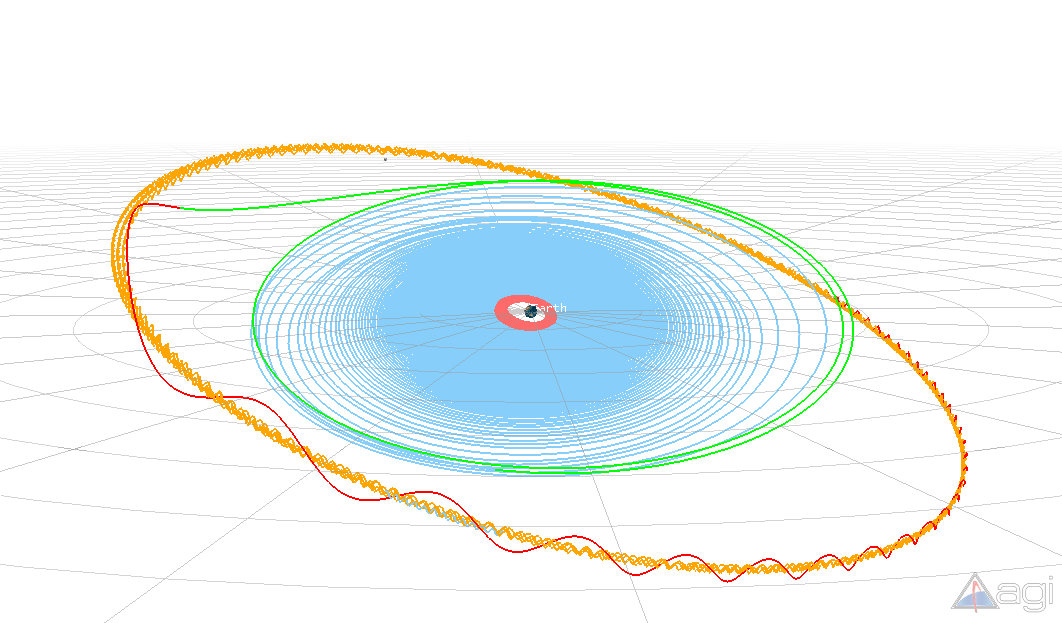
\includegraphics[width=\textwidth]{Images/STK/trajectory_white.png}
\caption{Continuous trajectory modelled in STK.} \label{fig:STK}
\end{figure}

Thus the STK simulation solves the problem of lunar capture, but further work was required to determine a feasible end-to-end orbit even before any optimisation could take place. In order to manipulate the thrust profile during the forwards ascent and cruise phases such that the initial GTO could connect with the lunar capture, it was necessary to reproduce this trajectory in GESOP. 

\subsection{Further GESOP modelling} \label{sub:GESOP2}

The ascent phase was modelled in GESOP subject to the initial boundary conditions outlined in \autoref{tab:Phase-2-constraints} and final boundary conditions outlined in \autoref{tab:Phase-2-3-constraints}. An initial guess was taken for the thrust profile perpendicular to the orbital radius at all times throughout ascent, in order to raise the periapsis as quickly as possible beyond the van Allen belts.

The initial guesses for starting time and mass were taken from the STK simulation described in \autoref{sec:STK}. End conditions were imposed to connect this phase to the starting conditions of the cruise phase. This implementation of continuity is not ideal as it enforces an arbitrary position and velocity at the phase transitions, thus reducing the flexibility during optimisation. A long-term goal remains to optimise all phases simultaneously, enforcing continuity between phases but not specifying what those conditions are. However at this stage this is not possible due to computational complexity, and remains an improvement for the future, perhaps exploiting parallel processing and supercomputer hardware.

Given the arbitrary nature of these continuity conditions, they were used for the initial guess but not enforced during optimisation. As the actual parameters diverged from their initial values during the optimisation, discontinuities emerged between phases. This was permitted for a number of reasons. Firstly, the launch conditions are not known, so the procedure used in this optimisation is more important than the actual result. Secondly, at every phase transition the terminating and commencing orbits are very similar, thus the variation in orbital energy was very small. In other words, the main difference between the orbits was simply timing, and at any of the phase transitions the spacecraft can sit in a parking orbit until the correct alignment occurs. Finally, due to the computational limitation of optimising each phase independently, any small change would then require all other phases to be recalculated. Treating each separately, with an implicit parking orbit in between, allows these small changes without any significant effect to the remaining phases.

As mentioned in \autoref{sec:Vehicle-power}, throughout the modelling and optimisation of the cruise phase, multiple different initial guesses were trialled. Ultimately it was decided that the initial specification for vehicle performance provided the best trajectory conditions, and consequently those same parameters were used in the STK simulation mentioned in \autoref{sec:STK}. The STK trajectory was then used as an initial guess for the cruise phase, subject to boundary conditions as outlined in \autoref{sec:BVP}. Once again, the cruise phase is not continuous with preceeding or succeeding phases, but the orbital energy at the phase boundaries is very similar allowing some design flexibility.

The $1.2\times10^6$ variables required to compute the cruise phase, as outlined in \autoref{sub:Discretisation}, resulted in $2\times10^8$ 64-bit doubles for floating point operations and $8\times10^7$ 32-bit words for integer operations. The desktop PC kindly provided by the Institute of Space Systems in Stuttgart, an AMD~2.8GHz~X6 with 2GB~RAM, was unable to handle a problem of this order. Despite an upgrade to 4GB, the cruise phase optimisation was still sluggish, resulting in the program terminating before it could achieve an optimal solution. The processing was severely restricted by not being distributed across the multiple cores available. To enable this, both GESOP and SOCS would have to be modified to support parallel processing. This would not only improve performance on desktop PCs given the market trend for multiple cores, but would allow large optimisation problems to be solved on clustered PCs, or even supercomputers. Unfortunately this development was beyond the scope of the project, so modelling proceeded to the remaining phases.

The initial mission architecture did not include a propagate phase, but during the STK simulation it was empirically found that the spacecraft achieves an appropriate orbit for lunar capture well before the Moon is in position for rendezvous. Consequently a coasting phase was inserted, when the spacecraft's trajectory was propagated forward in time without any thrusting. Given sufficient computational power, this phase could be shortened or removed entirely, much like the discontinuities between other phases, once the launch conditions are known. Whether this phase should be removed remains open to debate: it provides the spacecraft with an opportunity to recharge its batteries if the electrical system is not performing nominally, and allows time for critical adjustments if the spacecraft is drifting off course. The lunar approach is particularly important to ensure the final science phase orbit can be achieved without requiring too much propellant.

Throughout the propagate phase the spacecraft transitions from the Earth's sphere of influence to the Moon's. Consequently longitude was discarded in favour of time as the independent parameter for modelling this phase, as all the benefits outlined in \autoref{sec:Independent-parameter} are not applicable to this phase.

The various considerations of the phases introduced in \autoref{tab:Phases} are outlined in \autoref{tab:Phase-constraints}.

\begin{table}
\caption{.} \label{tab:Phase-constraints}
\begin{tabular}{l p{0.8\textwidth}} \toprule
Phase & Considerations \tabularnewline\midrule
Ascent & Earth-centred \tabularnewline
& Longitude as independent parameter \tabularnewline
Cruise & Earth-centred \tabularnewline
& Longitude as independent parameter \tabularnewline
Propagate & Earth-centred \tabularnewline
& Time as independent parameter \tabularnewline
Capture & Moon-centred \tabularnewline
& Time as independent parameter \tabularnewline
Descent & Moon-centred \tabularnewline
& Longitude as independent parameter \tabularnewline
Science & Moon-centred \tabularnewline
& Longitude as independent parameter \tabularnewline
\bottomrule
\end{tabular}
\end{table}

\subsection{Data analysis} \label{sub:Data-analysis}

During development, data was reviewed using the GESOP graphical interface. At the conclusion of work, the data files were imported into Matlab to produce the plots shown in this thesis. As explained in more detail in \autoref{sec:Validation}, the control and time vectors were post-processed in Matlab to fit the STK interface, to verify the orbital mechanics modelling.


%-----------------------------------------------------------------------------------------------------------------------------------------------------

% Final trajectory
\section{Final trajectory determination} \label{sec:Method-application}

The primary objective of this study was to determine a procedure for finding a suitable trajectory once the launch details are known. Launch configuration can be finalised before launch, but any launch can be postponed or scrubbed due to technical faults or even adverse weather. Therefore the trajectory can be approximated, but not finalised before launch. Once the spacecraft is safely in GTO, the orbital elements must be fed in to the optimisation process, and the resulting thrust profile uploaded to the spacecraft on-orbit. This procedure is graphically represented in \autoref{fig:Flowchart}.

\begin{figure}
\centering
\def\svgwidth{0.6\textwidth}
\input{Images/Flowchart.pdf_tex}
\caption{Flowchart demonstrating the trajectory development process for \BW.} \label{fig:Flowchart}
\end{figure}

First of all, the indicative results presented here may be used to estimate flight time, to produce a backward propagated trajectory in STK that departs GTO on a suitable date after launch. The capture and propagate phase durations may be adjusted to determine a lunar capture. Once a capture scenario is achieved, the state vector at each phase boundary must be inserted into GESOP as an initial guess prior to the optimisation process. 

The optimisation process within GESOP then commences. Given the present computational limitations, each phase must be optimised, then continuity conditions must be adjusted between phases. This iterative process is repeated until a smooth, continuous trajectory is achieved. Obviously, this process is sub-optimal. Assuming SOCS and GESOP have been adapted to support parallel processing, the phases may be appended into one large optimisation problem with many million parameters, which may then be optimised in one run.

Data files containing the control profile are output by GESOP. These may be post-processed, within GESOP or another application, to a format appropriate for the satellite AOCS, before being uploaded to the satellite. During the transfer the anticipated trajectory should be matched against the observed trajectory, and recalculated as required (this will be particularly important early in the trajectory, as thruster performance is evaluated).

\section{Summary} \label{sec:Method-summary}

This chapter clarified the software packages used throughout this project, and some of the problems inherent with each. A brief roadmap was then given to apply this procedure, after launch, to determine the final trajectory.

  
\clearpage